cumentclass[border=3pt,tikz]{standalone}
\usepackage{amsmath} % for aligned
\usetikzlibrary{arrows.meta} % for arrow size
\usepackage[outline]{contour} % glow around text
\contourlength{1.4pt}

% COLORS
\usepackage{xcolor}
\colorlet{myred}{red!80!black}
\colorlet{myblue}{blue!80!black}
\colorlet{mygreen}{green!60!black}
\colorlet{myorange}{orange!70!red!60!black}
\colorlet{mydarkred}{red!30!black}
\colorlet{mydarkblue}{blue!40!black}
\colorlet{mydarkgreen}{green!30!black}

% STYLES
\tikzset{
	>=latex, % for default LaTeX arrow head
	node/.style={thick,circle,draw=myblue,minimum size=22,inner sep=0.5,outer sep=0.6},
	node in/.style={node,green!20!black,draw=mygreen!30!black,fill=mygreen!25},
	node hidden/.style={node,blue!20!black,draw=myblue!30!black,fill=myblue!20},
	node convol/.style={node,orange!20!black,draw=myorange!30!black,fill=myorange!20},
	node out/.style={node,red!20!black,draw=myred!30!black,fill=myred!20},
	connect/.style={thick,mydarkblue}, 
	connect arrow/.style={-{Latex[length=4,width=3.5]},thick,mydarkblue,shorten <=0.5,shorten >=1},
	node 1/.style={node in}, % node styles, numbered for easy mapping with \nstyle
	node 2/.style={node hidden},
	node 3/.style={node out}
}
\def\nstyle{int(\lay<\Nnodlen?min(2,\lay):3)} % map layer number onto 1, 2, or 3
\pagecolor{gray!10} % Light gray background
\begin{document}
	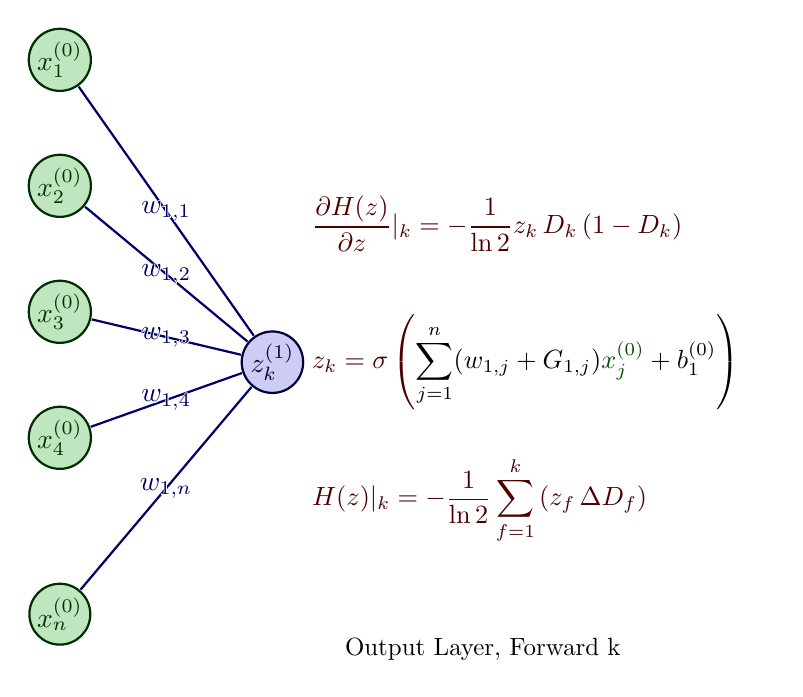
\begin{tikzpicture}[x=2.7cm,y=1.6cm]
		\message{^^JNeural network activation}
		\def\NI{5} % number of nodes in input layer
		\def\NO{1} % number of nodes in output layer (only z_1)
		\def\yshift{0.4} % shift last node for dots
		
		% INPUT LAYER
		\foreach \i [evaluate={\c=int(\i==\NI); \y=\NI/2-\i-\c*\yshift; \index=(\i<\NI?int(\i):"n");}]
		in {1,...,\NI}{ % loop over nodes
			\node[node in, outer sep=0.6] (NI-\i) at (0,\y) {$x_{\index}^{(0)}$};
		}
		
		% OUTPUT LAYER (only z_1)
		\foreach \i [evaluate={\c=int(\i==\NO); \y=\NO/2-\i-\c*\yshift; \index=(\i<\NO?int(\i):"n");}]
		in {1,...,\NO}{ % loop over nodes
			\ifnum\i=1 % highlighted node
			\node[node hidden, outer sep=0.6]
			(NO-\i) at (1,\y) {$z_{k}^{(1)}$};
			\foreach \j [evaluate={\index=(\j<\NI?int(\j):"n");}] in {1,...,\NI}{ % loop over nodes in previous layer
				\draw[connect,white,line width=1.2] (NI-\j) -- (NO-\i);
				\draw[connect] (NI-\j) -- (NO-\i)
				node[pos=0.50] {\contour{white}{$w_{1,\index}$}};
			}
			\fi
		}
		
			% ENTROPY EQUATION
		\node[below=-50,right=11,mydarkred,scale=0.95] at (NO-1) 
		{$\begin{aligned} 
				& \frac{\partial H(z)}{\partial z}|_k = - \frac{1}{\ln 2}  z_k\, D_k \left(1 - D_k \right)
			\end{aligned}$};
		
		% EQUATION LABEL
		\def\xgr#1{{\color{mydarkgreen}x_{#1}^{(0)}}} % green x_i^j for input layer
		\node[below=0,right=11,mydarkblue,scale=0.95] at (NO-1) 
		{$\begin{aligned} 
				& \color{mydarkred} z_k = \sigma\left( \color{black}
				\sum_{j=1}^{n} (w_{1,j} + G_{1,j}) \xgr{j}  + b_1^{(0)}\right)
			\end{aligned}$};
		
		% ENTROPY EQUATION
		\node[below=50,right=11,mydarkred,scale=0.95] at (NO-1) 
		{$\begin{aligned} 
				& H(z)|_k = - \frac{1}{\ln 2} \sum_{f=1}^{k} \left( z_f\, \Delta D_f \right)
			\end{aligned}$};
		
		% OUTPUT LAYER LABEL
		\node[below=40, right,scale=0.9] at (1.3,-2.3) {Output Layer, Forward k};
		
	\end{tikzpicture}
\end{document}
